%    Copyright (c)  2024  João Augusto Costa Branco Marado Torres.
%    Permission is granted to copy, distribute and/or modify this document
%    under the terms of the GNU Free Documentation License, Version 1.3
%    or any later version published by the Free Software Foundation;
%    with no Invariant Sections, no Front-Cover Texts, and no Back-Cover Texts.
%    A copy of the license is included in the section entitled "GNU
%    Free Documentation License".

%%%%%%%%%%%%%%%%%%%%%%%%%%%%% Define Article %%%%%%%%%%%%%%%%%%%%%%%%%%%%%%%%%%
\documentclass[a4paper,12pt]{article}
%%%%%%%%%%%%%%%%%%%%%%%%%%%%%%%%%%%%%%%%%%%%%%%%%%%%%%%%%%%%%%%%%%%%%%%%%%%%%%%

%%%%%%%%%%%%%%%%%%%%%%%%%%%%% Using Packages %%%%%%%%%%%%%%%%%%%%%%%%%%%%%%%%%%
\usepackage{geometry}
\usepackage{graphicx}
\usepackage{amssymb}
\usepackage{amsmath}
\usepackage{amsthm}
\usepackage{empheq}
\usepackage{mdframed}
\usepackage{booktabs}
\usepackage{lipsum}
\usepackage{graphicx}
\usepackage{color}
\usepackage{psfrag}
\usepackage{pgfplots}
\pgfplotsset{compat=1.18}
\usepackage{bm}
% % % % % % % % % % % % % % % % % % % % % % % % % % % % % % % % % % % % % % % %
\usepackage[utf8]{inputenc}
\usepackage[english]{babel}
\selectlanguage{english}
\usepackage{blindtext}
\usepackage{csquotes}
\usepackage{hyperref}
\hypersetup{colorlinks,
           %citecolor=black,
           %filecolor=black,
           %linkcolor=black,
           %urlcolor=black,
           bookmarksopen=true}
\usepackage[
backend=biber,
style=alphabetic,
sorting=ynt
]{biblatex}
\addbibresource{references.bib}
\usepackage{bookmark}
\usepackage{enumitem}
\usepackage{fancyhdr}
\pagestyle{fancy}
\fancyfoot[C]{\copyrightnotice}
\setlength{\headheight}{14.5pt}
%\addtolength{\topmargin}{-2.5pt}
\usepackage{mathtools}
\usepackage{tikz}
\usetikzlibrary{positioning,fit,calc}
\usepackage{float}
\usepackage{wrapfig}
%%%%%%%%%%%%%%%%%%%%%%%%%%%%%%%%%%%%%%%%%%%%%%%%%%%%%%%%%%%%%%%%%%%%%%%%%%%%%%%

% Other Settings

\pagenumbering{arabic}
\hfuzz = .6pt % avoid black boxes

%%%%%%%%%%%%%%%%%%%%%%%%%% Page Setting %%%%%%%%%%%%%%%%%%%%%%%%%%%%%%%%%%%%%%%
\geometry{a4paper}

%%%%%%%%%%%%%%%%%%%%%%%%%% Define some useful colors %%%%%%%%%%%%%%%%%%%%%%%%%%
\definecolor{ocre}{RGB}{243,102,25}
\definecolor{mygray}{RGB}{243,243,244}
\definecolor{deepGreen}{RGB}{26,111,0}
\definecolor{shallowGreen}{RGB}{235,255,255}
\definecolor{deepBlue}{RGB}{61,124,222}
\definecolor{shallowBlue}{RGB}{235,249,255}
%%%%%%%%%%%%%%%%%%%%%%%%%%%%%%%%%%%%%%%%%%%%%%%%%%%%%%%%%%%%%%%%%%%%%%%%%%%%%%%

%%%%%%%%%%%%%%%%%%%%%%%%%% Define an orangebox command %%%%%%%%%%%%%%%%%%%%%%%%
\newcommand\orangebox[1]{\fcolorbox{ocre}{mygray}{\hspace{1em}#1\hspace{1em}}}
%%%%%%%%%%%%%%%%%%%%%%%%%%%%%%%%%%%%%%%%%%%%%%%%%%%%%%%%%%%%%%%%%%%%%%%%%%%%%%%

\newcommand{\copyrightnotice}{
    Copyright \copyright{}  2024  João Augusto Costa Branco Marado Torres.
}
\newcommand{\licensenotice}{
    \copyrightnotice
    Permission is granted to copy, distribute and/or modify this document
    under the terms of the GNU Free Documentation License, Version 1.3
    or any later version published by the Free Software Foundation;
    with no Invariant Sections, no Front-Cover Texts, and no Back-Cover Texts.
    A copy of the license is included in the section entitled ``GNU
    Free Documentation License''.
}

%%%%%%%%%%%%%%%%%%%%%%%%%%%% English Environments %%%%%%%%%%%%%%%%%%%%%%%%%%%%%
\newtheoremstyle{mytheoremstyle}{3pt}{3pt}{\normalfont}{0cm}{\rmfamily\bfseries}{}{1em}{{\color{black}\thmname{#1}~\thmnumber{#2}}\thmnote{\,--\,#3}}
\newtheoremstyle{myproblemstyle}{3pt}{3pt}{\normalfont}{0cm}{\rmfamily\bfseries}{}{1em}{{\color{black}\thmname{#1}~\thmnumber{#2}}\thmnote{\,--\,#3}}
\theoremstyle{mytheoremstyle}
\newmdtheoremenv[linewidth=1pt,backgroundcolor=shallowGreen,linecolor=deepGreen,leftmargin=0pt,innerleftmargin=20pt,innerrightmargin=20pt,]{theorem}{Theorem}[section]
\theoremstyle{mytheoremstyle}
\newmdtheoremenv[linewidth=1pt,backgroundcolor=shallowBlue,linecolor=deepBlue,leftmargin=0pt,innerleftmargin=20pt,innerrightmargin=20pt,]{definition}{Definition}[section]
\theoremstyle{myproblemstyle}
\newmdtheoremenv[linecolor=black,leftmargin=0pt,innerleftmargin=10pt,innerrightmargin=10pt,]{problem}{Problem}[section]
%%%%%%%%%%%%%%%%%%%%%%%%%%%%%%%%%%%%%%%%%%%%%%%%%%%%%%%%%%%%%%%%%%%%%%%%%%%%%%%

%%%%%%%%%%%%%%%%%%%%%%%%%%%%%%% Plotting Settings %%%%%%%%%%%%%%%%%%%%%%%%%%%%%
\usepgfplotslibrary{colorbrewer}
\pgfplotsset{width=8cm,compat=1.9}
%%%%%%%%%%%%%%%%%%%%%%%%%%%%%%%%%%%%%%%%%%%%%%%%%%%%%%%%%%%%%%%%%%%%%%%%%%%%%%%

%%%%%%%%%%%%%%%%%%%%%%%%%%%%%%% Title & Author %%%%%%%%%%%%%%%%%%%%%%%%%%%%%%%%
\title{LANGuage IDentification}
\author{João Augusto Costa Branco Marado Torres}
%%%%%%%%%%%%%%%%%%%%%%%%%%%%%%%%%%%%%%%%%%%%%%%%%%%%%%%%%%%%%%%%%%%%%%%%%%%%%%%

\begin{document}
    \maketitle

    \section*{License}
    \bigskip
    \begin{quote}
        \licensenotice
    \end{quote}
    \bigskip

    \tableofcontents
    %\clearpage

    %\addcontentsline{toc}{chapter}{Foreword}
    %{\huge {\bf Foreword}}

    % \Blindtext

    \listoffigures
    %\listoftables

    \section{Phrases to Numeric Representation}

    I was really confused about this, but it really is not that complicated.

    Before starting to write any code, I wanted to know how can I transform a
    phrase like the one you are reading right now into \texttt{1}s and
    \texttt{0}s because the computer isn't smart enough to know English.
    So I went to my friend and
    \href{https://chatgpt.com/share/675976d6-b2c8-8002-964c-a3fff698bcc0}{asked
    it some questions}.
    It thought me various ways of achieving what I wanted, and between those
    options I picked the easiest to understand/implement.

    \subsection{Bag of Words}

    The idea it's to build a \textbf{vocabulary} which is a list of unique
    words.

    Everyone (including us) has its own vocabulary composed by words of the
    languages we speak.

    Our AI model needs a vocabulary too so he can understand some words. Those
    words might not exist in our vocabulary.

    Let's say {our model's vocabulary}~\ref{tab:rainbow_model_vocab} are
    the words in English for the 7 colors in the rainbow.

    Each word in the vocabulary will have a numerical identifier.

    \begin{table}
        \caption{Rainbow model vocabulary}\label{tab:rainbow_model_vocab}
        \begin{center}
            \begin{tabular}[c]{l|l}
                \hline
                \multicolumn{1}{c|}{\textbf{ID}} &
                \multicolumn{1}{c}{\textbf{Word}} \\
                \hline
                0 & red \\
                1 & orange \\
                2 & yellow \\
                3 & green \\
                4 & cyan \\
                5 & blue \\
                6 & violet \\

                \hline
            \end{tabular}
        \end{center}
    \end{table}

    It makes sense for us for that identifiers to start at \texttt{0} and
    increment by \texttt{1} for each word.

    Now our model can represent our phrases into something it understands.

    \begin{quote}
        How?
    \end{quote}

    The question you just asked is represented as a zero column matrix with 7
    rows.

    The model will try to find words he knows from a phrase and represent it as
    a column matrix with rows the same as the amount of words in the
    vocabulary. Each entry represents a word in the vocabulary, here is why
    it's a good idea to identify the words as I said. The value of each entry
    can be a simple boolean that represent if a word is present in the phrase
    or not, or the amount of times the word appears in the phrase. The value
    really represents how important is the that word in the phrase.

    The phrase ``How?'' does not contain any words know by the model.

    The phrase ``The colors in the \textit{Guiné-Bissau} flag are red, yellow,
    green and black in the star.'' would be represented by the matrix
    $\begin{bsmallmatrix}1&0&1&1&0&0&0\end{bsmallmatrix}^T$ and the phrase
    ``What came first, the orange fruit or the orange color?'' could be
    represented by $\begin{bsmallmatrix}0&2&0&0&0&0&0\end{bsmallmatrix}^T$ if
    we count the amount of occurrences of the word in the phrase.

    The way I implemented the BoW was by reading a file and collect every
    single word from it separated by white spaces, dashes, punctuation,
    parenthesis or quotation marks and then spit to \texttt{stdout} a formatted
    vocabulary, so you can pipe it later or write it to a file. Words are
    case-sensitive, and it's possible to create the vocabulary in alphabetic
    order.

    My implementation can be found in
    \href{run:../src/commands/vocab/bow.zig}{\texttt{/src/commands/vocab/bow.zig}}.

    During the conversation, ``tokenization'' was mentioned, and it might be
    cool for you to take a look at it.

    \subsection{Other ways}

    \begin{itemize}
        \item TF-IDF;
        \item One-Hot Encoding of Words;
        \item Embedding-like Approach;
        \item Sub-word tokenization.
    \end{itemize}

    \section{Neuron}

    As explained at the start of chapter 3.1 of \cite{bishop}, the base for the
    simplest supervised linear regression models will look like
    \eqref{eq:linear_model}
    \begin{equation}
        \begin{split}
            y(\mathbf{x}, \mathbf{w}) & = (1)b + w_{0}x_{0} + w_{1}x_{1} +
            \ldots + w_{D}x_{D} = \\ & = (1)b +
            \displaystyle\sum_{j=0}^{D}\left(w_{j}x_{j}\right)
        \end{split}
        \label{eq:linear_model}
    \end{equation}
    where $ \mathbf{x} =
    \begin{bsmallmatrix}x_{0}&\cdots&x_{D}\end{bsmallmatrix}^{T} $, a linear
    function of the parameters $ \mathbf{w} =
    \begin{bsmallmatrix}w_{0}&\cdots&w_{D}\end{bsmallmatrix} $ and bias $b$. We
    can also make the bias part of the $ \mathbf{w} $ and at the same position
    in $ \mathbf{x} $ put the value 1 and have the equation like
    \eqref{eq:linear_model_matrix}
    \begin{equation}
        y(\mathbf{x}, \mathbf{w}) = \mathbf{x}\cdot\mathbf{w}
        \label{eq:linear_model_matrix}
    \end{equation}
    a simple matrix multiplication. Both matrixes have the same amount of
    elements $ D $.

    There is also the notion of applying what is called as \textbf{basis
    function} to the $ \mathbf{x} $ parameters before everything. So there will
    be a matrix of basis functions $ \mathbf{\phi} =
    \begin{bsmallmatrix}\phi_{0}&\cdots&\phi_{D}\end{bsmallmatrix}^{T} $ where
    $ b = x_{i} $ and $ \phi_{i}(b) = 1 $.

    If that's the case the function will look like this
    \eqref{eq:linear_model_basis_f}
    \begin{equation}
        \begin{split}
            y(\mathbf{x}, \mathbf{w}) & =
            \displaystyle\sum_{j=0}^{D}\left(w_{j}\phi_{j}(x_{j})\right) = \\
            & = \mathbf{\phi}\left(\mathbf{x}\right)\cdot\mathbf{w}
        \end{split}
        \label{eq:linear_model_basis_f}
    \end{equation}

    The functions can be seen as a way to pre-process and extract the important
    parts of the input This list can have nonlinear functions making $
    y(\mathbf{x}, \mathbf{w}) $ nonlinear too.

    In case we are working with a classification model, we might want to
    introduce an \textbf{activation function} $ f\left(\cdot\right) $ that
    after all the computations in $ y(\mathbf{x}, \mathbf{w}) $
    \eqref{eq:linear_model_basis_f} transforms that result into a value
    corresponding to being the probability of $ \mathbf{x} $ being of a certain
    class.

    And this will be what I define as an artificial neuron \eqref{eq:neuron}.
    You can see a visual representation of it on page~\pageref{fig:neuron}

    \begin{equation}
        y(\mathbf{x}, \mathbf{w}) = f \left( \mathbf{\phi} \left( \mathbf{x}
        \right) \cdot\mathbf{w} \right)
        \label{eq:neuron}
    \end{equation}

    \begin{figure}
        \begin{center}
            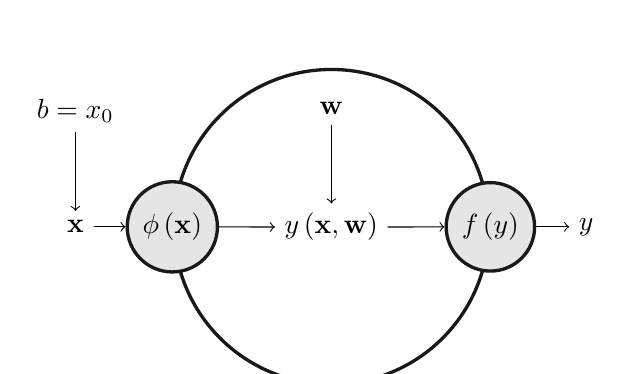
\begin{tikzpicture}[
                    neuron/.style={circle, draw=black!90, very thick},
                    var/.style={}, io/.style={circle, draw=black!90,
                    fill=black!10, very thick, minimum size=7mm},
                ]
                \node (neuron_logic) {$ y\left(\mathbf{x}, \mathbf{w}\right)
                $};
                \node (weights) [above=of neuron_logic] {$ \mathbf{w} $};
                \node[text opacity=0] (invisible) [below=of neuron_logic] {neuron};
                \node[neuron, fit={(weights)(neuron_logic)(invisible)}] (neuron) {};
                % \node[var] (input) [left=of neuron] {$ \mathbf{x} = \begin{bmatrix}x_{0}&x_{1}&\vdot&x_{D}\end{bmatrix} $};
                \node[var] (input) [left=of neuron] {$ \mathbf{x} $};
                \node[var] (bias) [above=of input] {$ b = x_{0} $};
                \node[var] (output) [right=of neuron] {$ y $};
                \node[io] (basis) at (neuron.west) {$
                \mathbf{\phi}\left(\mathbf{x}\right) $};
                \node[io] (activation) at (neuron.east) {$ f\left(y\right) $};

                \draw[->] (bias.south) -- (input.north);
                \draw[->] (input.east) -- (basis.west);
                \draw[->] (basis.east) -- (neuron_logic.west);
                \draw[->] (neuron_logic.east) -- (activation.west);
                \draw[->] (activation.east) -- (output.west);
                \draw[->] (weights.south) -- (neuron_logic.north);
            \end{tikzpicture}
        \end{center}
        \caption{A visual representation of a neuron.}\label{fig:neuron}
    \end{figure}

    Because I couldn't find a simple way of doing anonymous functions in my
    language of choice, \href{run:../src/utils/neuron.zig}{my implementation}
    does not allow specifying basis functions nor activation functions so every
    basis function can be thought as being the identify function $
    \mathbf{\phi}(x) = x $ and the activation function can be toggled between
    the identify and sigmoid \eqref{eq:sigmoid}.

    \begin{equation}
        \sigma\left(x\right) = \frac{1}{1+e^{-x}}
        \label{eq:sigmoid}
    \end{equation}

    %\section{Feed-Forward Neural Network}

    \medskip

    \printbibliography[
    heading=bibintoc
    ]

\end{document}
